\documentclass[12pt, twoside]{article}
\input{../preamble}

\fancyhead[LE]{\thepage}
\fancyhead[RO]{\thepage}
\fancyhead[LO]{La Scuola d'Italia / Dr.\ Huson / IB Math --- Early Finishers \\* 13 March 2026}

\begin{document}
\subsubsection*{4.18 Normal and Binomial Distribution}

\begin{enumerate}[itemsep=0.15cm]

%--- Problem 1: Simple Binomial ---
\item A bakery finds that 15\% of its croissants are overcooked.
      A box contains 10 randomly selected croissants.
      Let $X$ be the number of overcooked croissants in the box.

\begin{center}
\vspace{-0.3cm}
\begin{tikzpicture}[scale=0.55]
  \draw[-{Stealth}] (-0.8,0) -- (7,0) node[right] {$x$};
  \draw[-{Stealth}] (0,-0.5) -- (0,4.5) node[above] {$\mathrm{P}(X=x)$};
  \foreach \x/\h in {0/1.97, 1/3.47, 2/2.76, 3/1.30, 4/0.40, 5/0.08} {
    \fill[gray!30] (\x-0.35,0) rectangle (\x+0.35,\h);
    \draw (\x-0.35,0) rectangle (\x+0.35,\h);
  }
  \foreach \x in {0,...,5} \draw (\x,0.1)--(\x,-0.1) node[below]{\small\x};
  \foreach \y/\l in {1/0.1, 2/0.2, 3/0.3}
    {\draw (0.1,\y)--(-0.1,\y) node[left]{\small\l};}
\end{tikzpicture}
\vspace{-0.3cm}
\end{center}

\begin{enumerate}[itemsep=0.1cm]
  \item Find the expected number of overcooked croissants in a box, $E(X)$. \hfill [1]
  \item Find the probability that none of the croissants are overcooked. \hfill [2]
   \item Find the probability that at most 1 croissant is overcooked. \hfill [2]
  \item Find $\mathrm{P}(X = 2)$. \hfill [2]
  \item Find $\mathrm{P}(X \leq 1)$. \hfill [2]
\end{enumerate}

\vfill

%--- Problem 2: Simple Normal ---
\item The heights of sunflower plants in a garden follow a normal distribution
      with mean $\mu = 145$\,cm and standard deviation $\sigma = 12$\,cm.
\vspace{0.5cm}

\begin{center}
\vspace{-0.3cm}
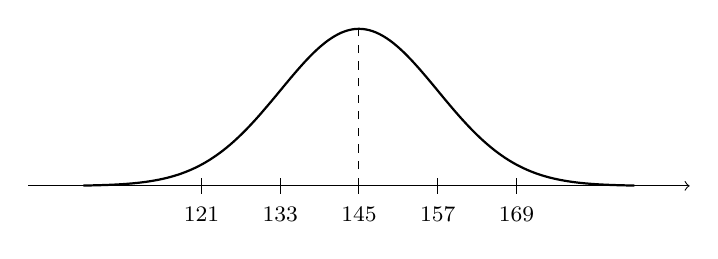
\begin{tikzpicture}[xscale=1, yscale=5]
  \draw[->] (-4.2,0) -- (4.2,0);
  \draw[thick, smooth, domain=-3.5:3.5, samples=80]
    plot (\x, {exp(-0.5*\x*\x)/2.507});
  \draw[dashed] (0,0) -- (0,0.399);
  \foreach \v/\l in {-2/121, -1/133, 0/145, 1/157, 2/169}
    {\draw (\v,0.02)--(\v,-0.02); \node[below] at (\v,-0.03) {\footnotesize\l};}
\end{tikzpicture}
\vspace{-0.3cm}
\end{center}

\begin{enumerate}[itemsep=0.1cm]
  \item Find the probability that a randomly selected plant is taller
        than 160\,cm. \hfill [2]
  \item Find the probability that a plant's height is between
        130\,cm and 155\,cm. \hfill [2]
  \item 80\% of the plants are shorter than $h$\,cm. Find $h$. \hfill [3]
\end{enumerate}

\vfill

\newpage

%--- Problem 3: Combined Normal + Binomial ---
\item The time $T$ (minutes) for a commuter train journey follows a normal
      distribution with mean 48 minutes and standard deviation $\sigma$ minutes.
      It is known that 5\% of journeys take longer than 55 minutes.

\begin{enumerate}[itemsep=0.3cm]
  \item Find the value of $\sigma$. \hfill [3] \vspace{2cm}
  \item Find $\mathrm{P}(T < 42)$. \hfill [2] \vspace{2cm}
  \item On a particular day, 20 journeys are made. Find the probability that
        \\at most 2 of these journeys take less than 42 minutes. \hfill [3] \vspace{4cm}
  \item A journey is selected at random. Given that it took less than
        52 minutes, \\find the probability that it took less than
        42 minutes. \hfill [3]
\end{enumerate}

\vfill

\end{enumerate}
\end{document}

Solutions
  Problem 1 — Binomial, X ~ B(10, 0.15):
  - (a) X ~ B(10, 0.15)
  - (b) P(X=2) = binomPdf(10, 0.15, 2) = 0.27590... ≈ 0.276
  - (c) P(X≤1) = binomCdf(10, 0.15, 0, 1) = 0.54432... ≈ 0.544

  Problem 2 — Normal, H ~ N(145, 12²):
  - (a) P(H > 160) = normCdf(160, 1E99, 145, 12) = 0.10565... ≈ 0.106
  - (b) P(130 < H < 155) = normCdf(130, 155, 145, 12) = 0.69195... ≈ 0.692
  - (c) h = invNorm(0.80, 145, 12) = 155.099... ≈ 155

  Problem 3 — Combined Normal + Binomial, T ~ N(48, σ²):
  - (a) P(T > 55) = 0.05: invNorm(0.95) = 1.6449; σ = 7/1.6449 = 4.2555... ≈ 4.26
  - (b) P(T < 42) = normCdf(0, 42, 48, 4.2555) = 0.07930... ≈ 0.0793
  - (c) Y ~ B(20, 0.0793): P(Y ≤ 2) = binomCdf(20, 0.0793, 0, 2) = 0.7798... ≈ 0.780
  - (d) P(T<42|T<52) = P(T<42)/P(T<52) = 0.07930/0.82633 = 0.09597... ≈ 0.0960
